\section{Related Works}
\begin{frame}{Related Works}
\framesubtitle{Shallow methods}
\begin{itemize}
\item Early approach to the Text Classification problem using rule-based systems where an expert suggests a rule for classifying text, based on the semantics and pragmatics of the data. 

\item Later on, several methods with the concept of using the probability of tokens to predict if a document belongs
to a specific class were proposed:
\begin{itemize}
\item Na\"ive Bayes\cite{Xu2017}
\item Decision Trees\cite{Safavian1991}
\item Logistic Regression\cite{Genkin2007}
\item Support Vector Machine (SVM)\cite{boser1992, cortesvapnik1995}.
\end{itemize}
\end{itemize}
\end{frame}

\begin{frame}{Related Works (cont.)}
\framesubtitle{Deep methods -- Sequence-to-Sequence (Seq2Seq)}
The Sequence-to-Sequence (Seq2Seq) architecture were introduced by Sutskever et al. (2014)\cite{Sutskever2014}. We can modify the original Seq2Seq architecture to create a text classification model, using context from the Encoder.
\begin{columns}
\begin{column}{.5\textwidth}
\begin{figure}
\centering
\resizebox{\linewidth}{!}{
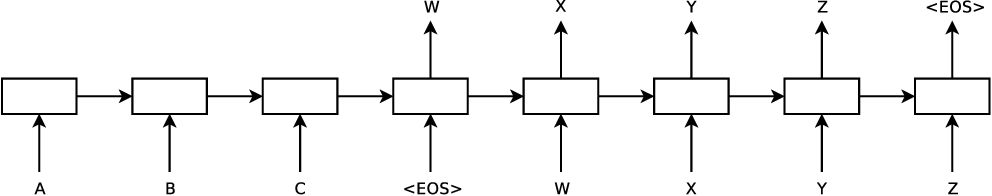
\includegraphics{img/seq2seq.png}
}
\caption{The original Seq2Seq model proposed by Sutskever et al. (2014) for Machine Translation task\cite{Sutskever2014}.}
\end{figure}
\end{column}
\begin{column}{.5\textwidth}
\begin{figure}
\centering
\resizebox{\linewidth}{!}{
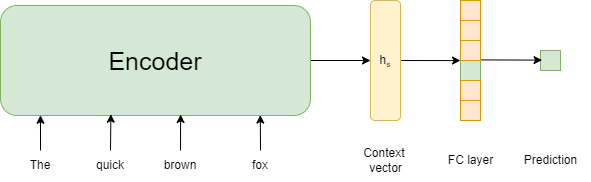
\includegraphics{img/seq2seq-classification.png}
}
\caption{Example for a modified Seq2Seq model for Text Classification task}
\end{figure}
\end{column}
\end{columns}
\end{frame}

\begin{frame}{Related Works (cont.)}
\framesubtitle{Deep methods -- CNN}
Kim et al. (2014)\cite{Kim2014} used CNN with different filter sizes to build an efficient architecture for Text Classification.
\begin{figure}
\centering
\resizebox{\linewidth}{!}{
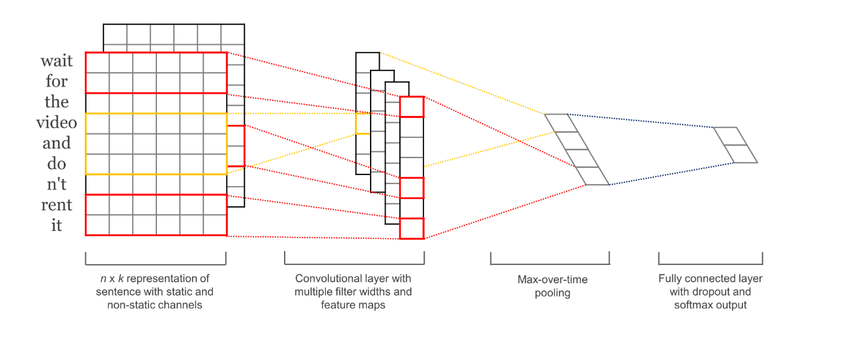
\includegraphics{img/cnn-classification.png}
}
\caption{The CNN architecture for Text Classification task by Kim et al. (2014)\cite{Kim2014}}
\end{figure}
\end{frame}

\begin{frame}{Related Works (cont.)}
\framesubtitle{Deep methods -- Multi-channel CNN and LSTM}
Vo et al. (2017)\cite{Vo2017} proposed a method combines CNN and recurrent networks such as LSTM for Vietnamese Text Classification.
\begin{figure}
\centering
\resizebox{\linewidth}{!}{
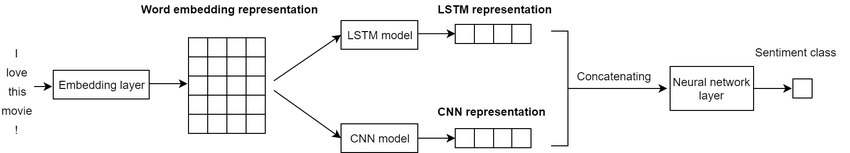
\includegraphics{img/CNN-LSTM-ensemble.png}
}
\caption{The Multi-channel CNN and LSTM architecture for Text Classification task by Vo et al. (2017)\cite{Vo2017}}
\end{figure}
\end{frame}

\begin{frame}{Related Works (cont.)}
\framesubtitle{Deep methods -- Large Language Models (LLMs)}
Recently, deep large language models (LLMs -- e.g. BERT\cite{Devlin2019}, RoBERTa\cite{Liu2019}, XLM\cite{Conneau2020}, ..etc) have shown state-of-the-art performance on many text classification tasks. These models are highly scalable, making them suitable for processing large amounts of text data.

\begin{figure}
\centering
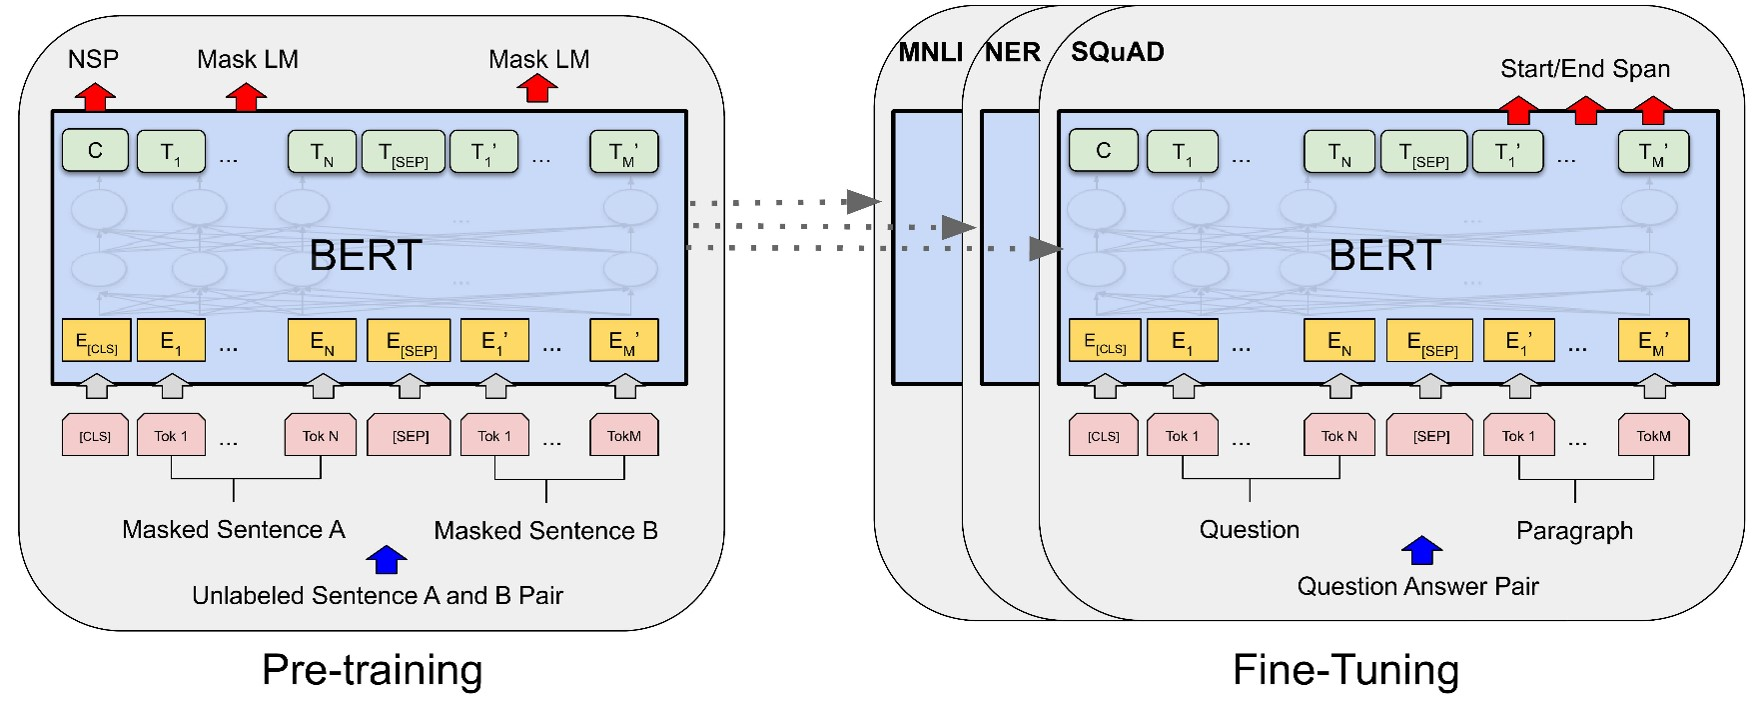
\includegraphics[scale=.5]{img/BERT.jpg}
\caption{The BERT architecture by Devlin et al. (2019)\cite{Devlin2019}}
\end{figure}
\end{frame}